\documentclass{report}

\usepackage[left=3cm,right=3cm,top=1cm,bottom=2cm]{geometry}
\usepackage{polski}
\usepackage[utf8]{inputenc}
\usepackage{graphicx, float}

\newenvironment{absolutelynopagebreak}
{\par\nobreak\vfil\penalty0\vfilneg
	\vtop\bgroup}
{\par\xdef\tpd{\the\prevdepth}\egroup
	\prevdepth=\tpd}

\title{%
	System pisania testów na platformie Android \\
	\large Raport inżynierski}

\author{
	Filip Malinowski\\
	\texttt{filip.malinowski@student.pwr.edu.pl}
	\and
	pod przewodnictwem Promotora dr Witolda Paluszyńskiego\\
	\texttt{witold.paluszynski@pwr.edu.pl}
}
\date{}

\begin{document}

%\maketitle

	\chapter{Przegląd zagadnień}

	Tematem pracy jest stworzenie systemu na platformę Android umożliwiającego pisanie testów na wykładach akademickich i zautomatyzowane przetworzenie wyników testów. W skład systemu planowo mają wejść: aplikacja na system Android oraz aplikacja serwerowa, z którą aplikacja połączy się wysyłając wybrane przez użytkownika odpowiedzi.\\
	
	Na rynku istnieją już aplikacje częściowo odpowiadające tematowi pracy inżynierskiej. Ich funkcjonalność spełnia pewne aspekty jakimi są: wybór odpowiedzi, przesyłanie odpowiedzi do serwera oraz pobieranie treści z serwera na aplikację. Najlepszym przykładem jest aplikacja nazywająca się Quizowanie \footnote{https://play.google.com/store/apps/details?id=se.feomedia.quizkampen.pl.lite}. Aplikacja ta pozwala na pobieranie i wyświetlenie pytań z serwera, wyświetlenie możliwych odpowiedzi jako przycisków dla użytkownika oraz wysłanie odpowiedzi do serwera i zweryfikowanie ich. Jej kod źródłowy jest jednak zamknięty co sprawia, że jest nieprzydatny przy tworzeniu systemu będącego tematem tej pracy.
	
	Inne aplikacje, które można wymienić to English Grammar Test\footnote{https://play.google.com/store/apps/details?id=english.grammar.test.app} lub też sameQuizy\footnote{https://play.google.com/store/apps/details?id=pl.filing.samequizy}. Ich wartość ogranicza się jednak do rozwiązań dotyczących wyglądu interfejsu aplikacji. Nie ma możliwości w legalny sposób uzyskać kodu źródłowego lub opisów rozwiązań w tych aplikacjach z racji ich komercyjnego zastosowania.
	\\
	W przypadku aplikacji serwerowej jest wiele możliwych technologii, które można zastosować przy jej tworzeniu. Pierwszym etapem był wybór protokołu komunikacyjnego jaki zostanie użyty między aplikacją androidową, a serwerem. Możliwe protokoły to np. TCP, UDP, POP, SMTP, HTTP czy FTP. Wybrany został protokół HTTP z powodu tego, że sieć WiFi na Politechnice Wrocławskiej ma odblokowaną komunikację na portach 80 oraz 8080 oraz prawdopodobnie na tych wymienionych portach sprawdzane są też użyte protokoły i ich zgodność z HTTP. Innego rodzaju protokół wykluczyłby użycie systemu w połączeniu z politechniczną siecią WiFi co znacząco obniżyłoby jego zastosowanie.
	
	Kolejnym etapem był wybór odpowiedniego odpowiedniego serwera web do obsługi zapytań przesłanych z aplikacji mobilnej. Możliwe aplikacje serwerowe jakie można wykorzystać to: Apache, nginx, lighttpd, OpenLiteSpeed. Początkowe wersje aplikacji mobilnej komunikują się z serwerem Apache\footnote{https://httpd.apache.org/} jednak docelowo ma zostać do tego użyty nginx\footnote{https://www.nginx.com/}. Z racji tego, że większość serwerów obsługuje FastCGI pozwalających na napisanie programu obsługującego zapytania w wielu popularnych językach, to przy wyborze serwera kierowano się jego wydajnością obsługi zapytań przychodzących. Wykorzystano tutaj Linux Web Server Performance Benchmark\footnote{https://www.rootusers.com/linux-web-server-performance-benchmark-2016-results/} z 2016.
	
	
	\begin{center}
		\begin{figure}[ht]
			\centering
			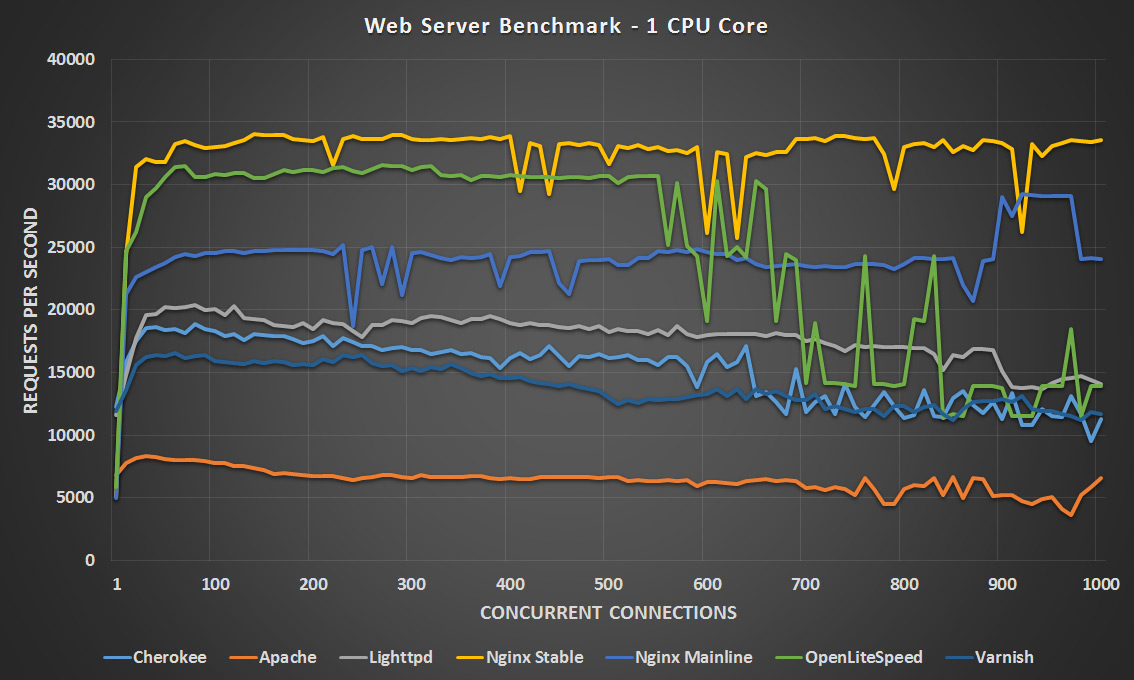
\includegraphics[scale=0.3]{web-server-performance-benchmark-1-cpu-core-1.jpg}
			\caption{Wykres przedstawiający ilość obsługiwanych zapytań przy danej ilości otwartych połączeń z Linux Web Server Performance Benchmark}
		\end{figure}
	\end{center}
	
	
	Należało też wybrać środowisko w jakim aplikacja mobilna powinna powstać. W tym przypadku do wyboru jest Android Studio\footnote{https://developer.android.com/studio/index.html} oraz Qt\footnote{https://www.qt.io/}. Oba środowiska oferują duże wsparcie ze strony społeczności programistycznej oraz szeroki zestaw narzędzi. Oba pozwalają na tworzenie interfejsu użytkownika w XML oraz udostępniają klasy obiektów przydatne do wizualizowania i przetwarzania danych. Wybrany został jednak Android Studio z racji jego największej popularności oraz najszerszej gamy narzędzi wchodzących w skład tego środowiska. Pozwala na dołączanie bibliotek z repozytoriów Git lub też bibliotek za pomocą wbudowanego narzędzia Maven\footnote{https://maven.apache.org/}, bieżące sprawdzanie kompatybilności użytych bibliotek z wersjami systemu Android na które aplikacja powstaje oraz tworzenie maszyn wirtualnych do testowania napisanych aplikacji.
	\\
	Zważywszy na powyżej przedstawione informacje system do rozwiązywania testów musi być napisany od podstaw. Nie znaleziono przykładów otwartych systemów na tyle użytecznych, żeby można było użyć ich przy tworzeniu systemu. Systemy takie jak Quizowanie mają zamknięty kod i można się nimi sugerować jedynie w kwestii tworzenia interfejsu użytkownika.
	
	W trakcie pracy nad systemem do rozwiązywania testów wymagania co do tego systemu zostały doprecyzowane. Aplikacja mobilna musi być przyjazna dla użytkownika i intuicyjna. Użytkownik dalej ma możliwość pisania testów na papierze dlatego forma elektroniczna musi być wystarczająco zachęcająca. Ponadto musi też być niezawodna. Nie powinna tracić przetwarzanych w niej istotnych informacji lub wyłączać się w trakcie rozpoczęcia pisania testu. Aplikacja musi się też w niezawodny sposób łączyć z serwerem w celu przesłania odpowiedzi użytkownika lub też pozwolić na ponowne ich wysłanie po utracie połączenia. Kopie zapasowe testów muszą też być zapisywane w pamięci wewnętrznej telefonu, a ich zawartość zaszyfrowana chroniąc wrażliwe dane przed ingerencją osób nieupoważnionych. Aplikacja powinna też być weryfikowalna przez serwer, żeby nie dopuścić do wysyłania odpowiedzi aplikacji zmodyfikowanych przez osoby trzecie. Musi też informować użytkownika odpowiednimi komunikatami wyświetlanymi na ekranie o zaistniałych problemach na każdym etapie użytkowania, żeby użytkownik wiedział w jaki sposób reagować na nieprzewidziane sytuacje.
	
	Aplikacja serwerowa musi być w stanie obsługiwać sprawnie wysoki ruch, w którym przybywa średnio 10 zapytań na sekundę dochodzących nawet do 100 na sekundę przy 100 osobowej grupie użytkowników piszących na aplikacji test. Docelowo powinna jednak być w stanie obsłużyć nawet 300-400 użytkowników, żeby można było ją zastosować w każdej możliwej grupie studentów na Politechnice Wrocławskiej. Serwer musi też być w stanie weryfikować łączące się aplikacje, tak aby nie przesyłać wrażliwych informacji do nieupoważnionych osób. Jego struktura musi być możliwie prosta, żeby przyszłe modyfikacje były mało uciążliwe dla użytkownika całego systemu.
	\\
	
	\chapter{Stopień zaawansowania prac}
	
	Aplikacja mobilna przechowuje dane użytkownika takie jak: Imię, Nazwisko, numer indeksu oraz nazwa przedmiotu na którym wykonywany jest test. Umożliwia też zmianę adresu serwera, na który przysyłane są odpowiedzi z testu. Dane te zmienia się w ustawieniach aplikacji. W menu głównym pozwala na wprowadzenie rzędu i miejsca, na którym użytkownik siedzi podczas testu, wektora wag służącego do obliczania grupy oraz ID testu jaki jest przeprowadzany. Zostało też zaimplementowane udogodnienie dla użytkownika w postaci skanera kodów QR umożliwiającego zautomatyzowane wczytanie wektora wag, ID testu i wyliczenie grupy użytkownika. Do skanowania kodów QR została wykorzystana biblioteka zxing\footnote{https://github.com/zxing/zxing} (Zebra Crossing). Po przejściu do testu wyświetlany jest ekran konfiguracyjny aplikacji gdzie użytkownik jest informowany o operacjach przeprowadzanych przed rozpoczęciem testu. Na obecnym etapie prac aplikacja sprawdza osiągalność serwera, do którego wysyła odpowiedzi oraz pobiera plik konfiguracyjny zawierający takie dane jak minimalna i maksymalna wersja aplikacji dopuszczona do testu oraz klucz szyfrowania danych w plikach testu przechowywanych na telefonie użytkownika. Po przejściu do testu wyświetlana jest zakładka pytania, a na niej: nr grupy w jakiej użytkownik się znajduje, nr pytania, przyciski do wysłania odpowiedzi "tak", "nie", "nie wiem"; przyciski do dodania pytania i do podsumowania testu oraz unikalny identyfikator sesji wygenerowany dla aktualnej sesji testowej otwartej na telefonie. Dodanie pytania wymusza przejście do następnego pytania a UI użytkownika pozwala na przesuwanie ekranu w celu dostania się do innych pytań. Podsumowanie testu wyświetla ilość poprawnie przesłanych odpowiedzi "tak", "nie" oraz "nie wiem" do serwera, oraz ilość odpowiedzi zapisanych w pliku testowym. W razie różnicy w odpowiedziach przesłanych do serwera a zapisanych w pliku aplikacja wyświetla odpowiednie ostrzeżenie sugerujące użytkownikowi powrót do testu i ponowne przesłanie odpowiedzi. Na ekranie podsumowania wyświetlany jest przycisk pozwalający powrót do testu oraz przycisk kończący test powodujący powrót do menu głównego aplikacji.
	
	Obecnie serwerem do obsługi zapytań sieciowych jest Apache. Do przetwarzania danych wykorzystano skrypt napisany w języku AWK. Skanuje on logi serwera Apache w poszukiwaniu zarejestrowanych zapytań przysłanych z aplikacji mobilnych i umożliwia zapisanie ich w formacie użytecznym dla użytkownika całego systemu.
	
	Stworzony został też deszyfrator plików przechowywanych na telefonach użytkowników pozwalający na odzyskanie odpowiedzi w razie problemów z połączeniem z serwerem gdy nie wszystkie odpowiedzi do niego dotarły.
	
	Do tworzenia plików konfiguracyjnych stworzony został konfigurator. Tworzy on dokument XML zawierający klucz szyfrowania i zakres dopuszczalnych wersji aplikacji, oraz tworzy on plik przechowujący klucz do deszyfrowania.
	
	\chapter{Elementy aplikacji}
	
		\section{Widoki aplikacji}
		
		Wygląd aplikacji stanowi ważny element aplikacji. W początkowych fazach projektu rozmieszczenie elementów na ekranie telefonu komórkowego jak też ich estetyka wielokrotnie była zmieniana. Potrzebne było wypracowanie przejrzystego oraz przyjaznego dla studenta interfejsu aplikacji. W trakcie tworzenia aplikacji zauważono, że istotnym elementem jest zachowanie kompatybilności z różnymi wersjami systemu Android realizując jednolite i przewidywalne zachowanie się interfejsu aplikacji.
		Na przykład nie można było zastosować kolorowania przycisków korzystając z metody setColorFilter obecnej we wszystkich wersjach systemu od Android 4.0 do Android 7.0. Wywołanie tej metody w systemach Android 4.0 do 4.4 powodowało zakolorowanie przycisku w sposób ujawniający się dopiero po odtworzeniu widoku. W systemach Android 5.0 i wyższych powodowało natychmiastową zmianę koloru przycisku.
		Widoki jakie zostały zaimplementowane w aplikacji to:
		\begin{itemize}
			\item Widok główny\\
			\begin{minipage}{0.45\textwidth}
				Za jego pomocą użytkownik może wprowadzić swoje miejsce i rząd w jakim się znajduje, wektor wag służący do wyliczenia grupy na teście oraz kod testu. Na tym widoku można uruchomić również skaner kodów QR do automatycznego pobrania wektora wag i kodu testu oraz wyliczenia grupy na teście. Trzy dolne przyciski służą do wyjścia z aplikacji, ręcznego wyliczenia numeru grupy oraz przejścia do testu. Z tego widoku można również otworzyć menu, z którego można dostać się do widoku ustawień i widoku informacji.
			\end{minipage}
			\begin{minipage}{0.5\textwidth}
				\begin{figure}[H]
					\begin{center}
					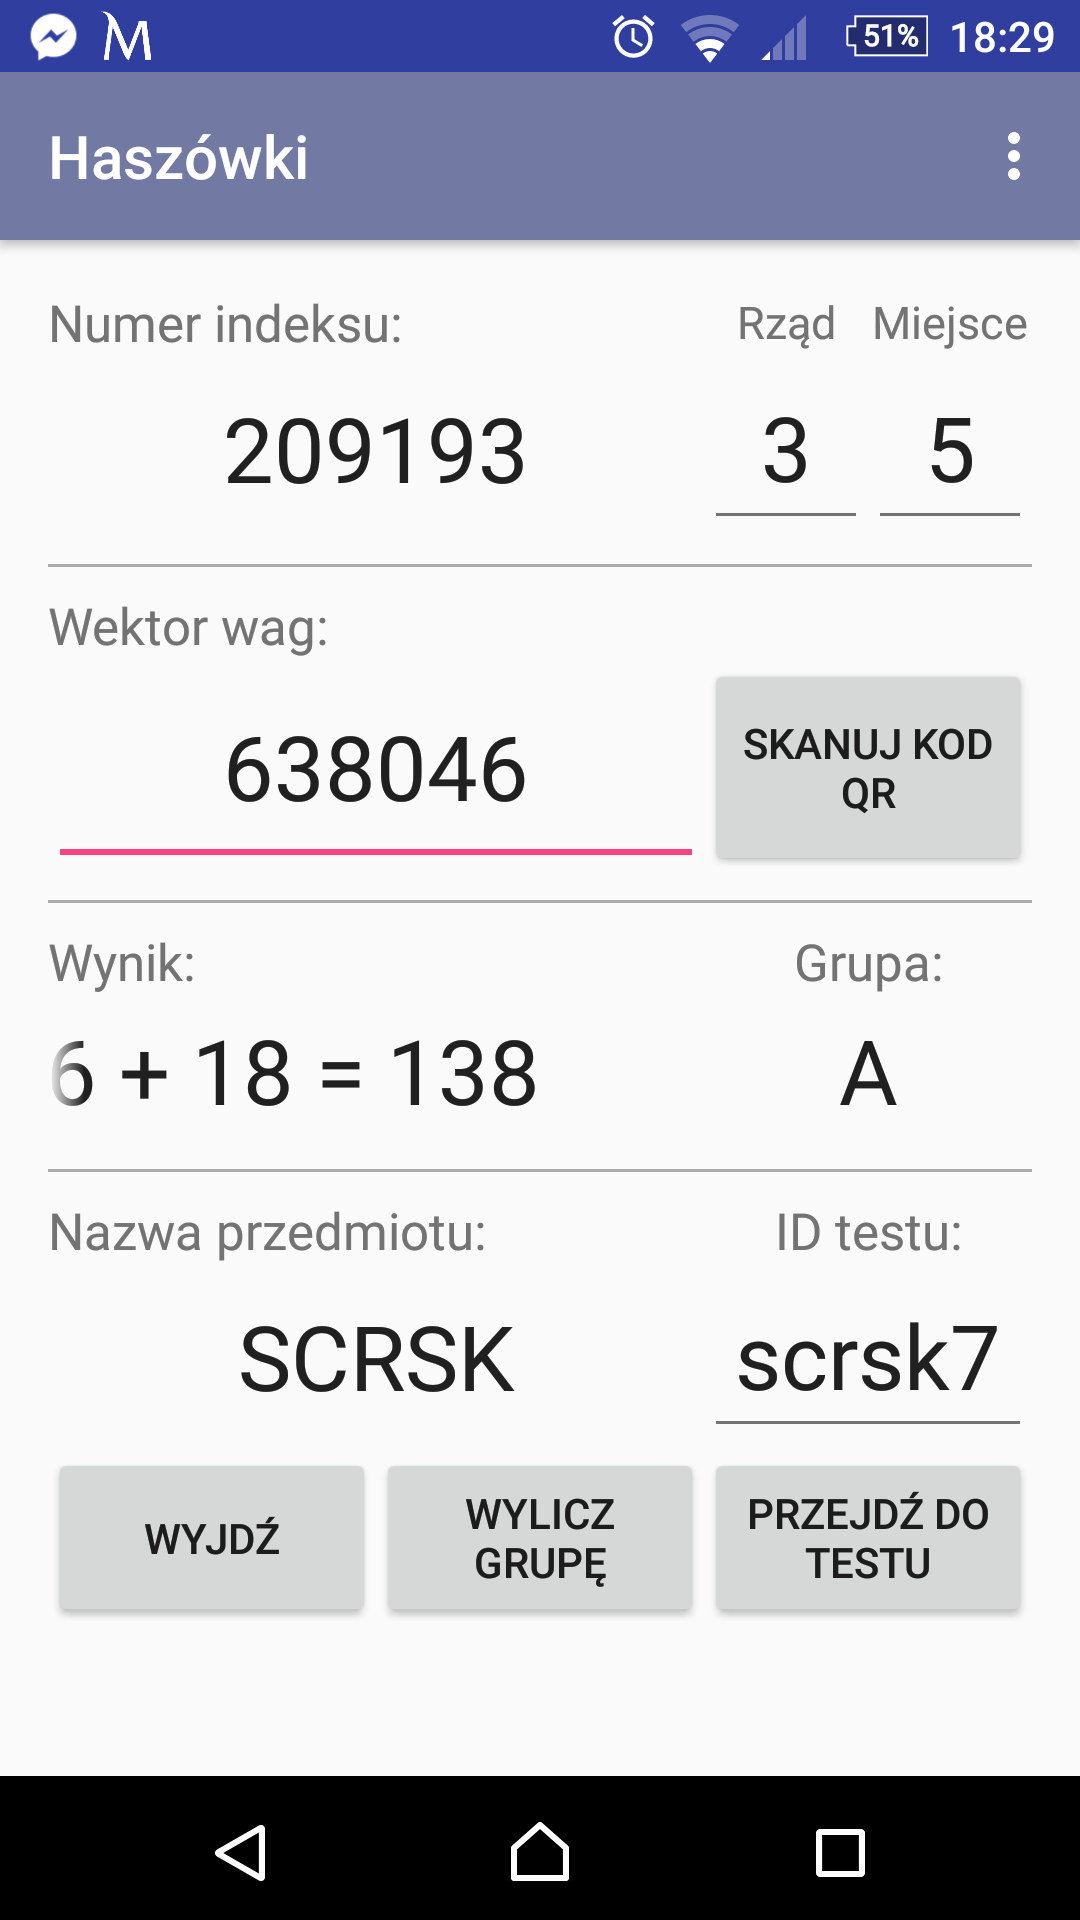
\includegraphics[scale=0.1]{widok_glowny}
					\end{center}
				\end{figure}
			\end{minipage} \hfill
			
			\pagebreak
			
			\item Widok ustawień\\
			\begin{minipage}{0.45\textwidth}
			Tutaj użytkownik może wprowadzić i zapisać w aplikacji swoje dane takie jak: imię, nazwisko, numer indeksu oraz nazwa przedmiotu. Opcjonalnie może wprowadzić inny adres serwera, na który aplikacja będzie przesyłać odpowiedzi użytkownika.
			\end{minipage}
			\begin{minipage}{0.5\textwidth}
				\begin{figure}[H]
					\begin{center}
					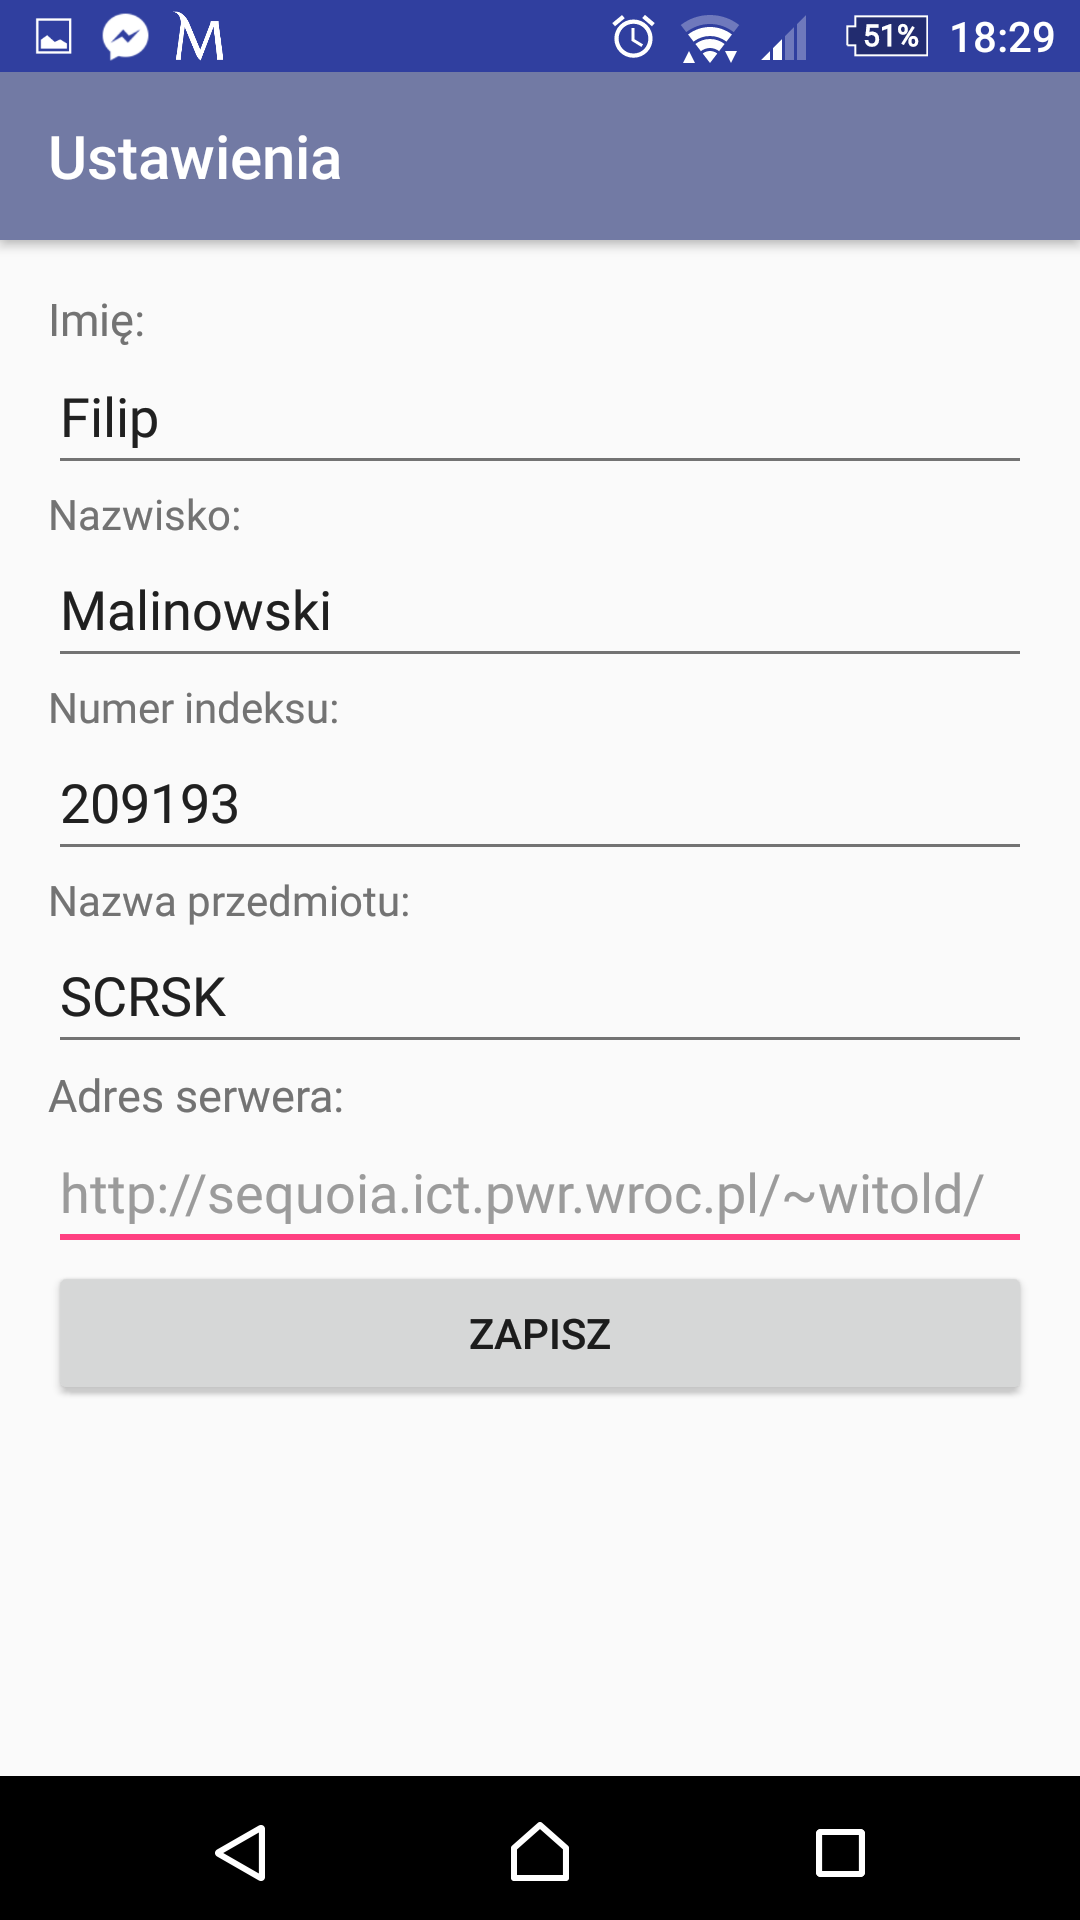
\includegraphics[scale=0.1]{widok_ustawien}
					\end{center}
				\end{figure}
			\end{minipage} \hfill
			
			\item Widok informacji\\
			\begin{minipage}{0.45\textwidth}
			W tym widoku użytkownik może się dowiedzieć z jakiej wersji aplikacji korzysta.
			\end{minipage}
			\begin{minipage}{0.5\textwidth}
				\begin{figure}[H]
					\begin{center}
					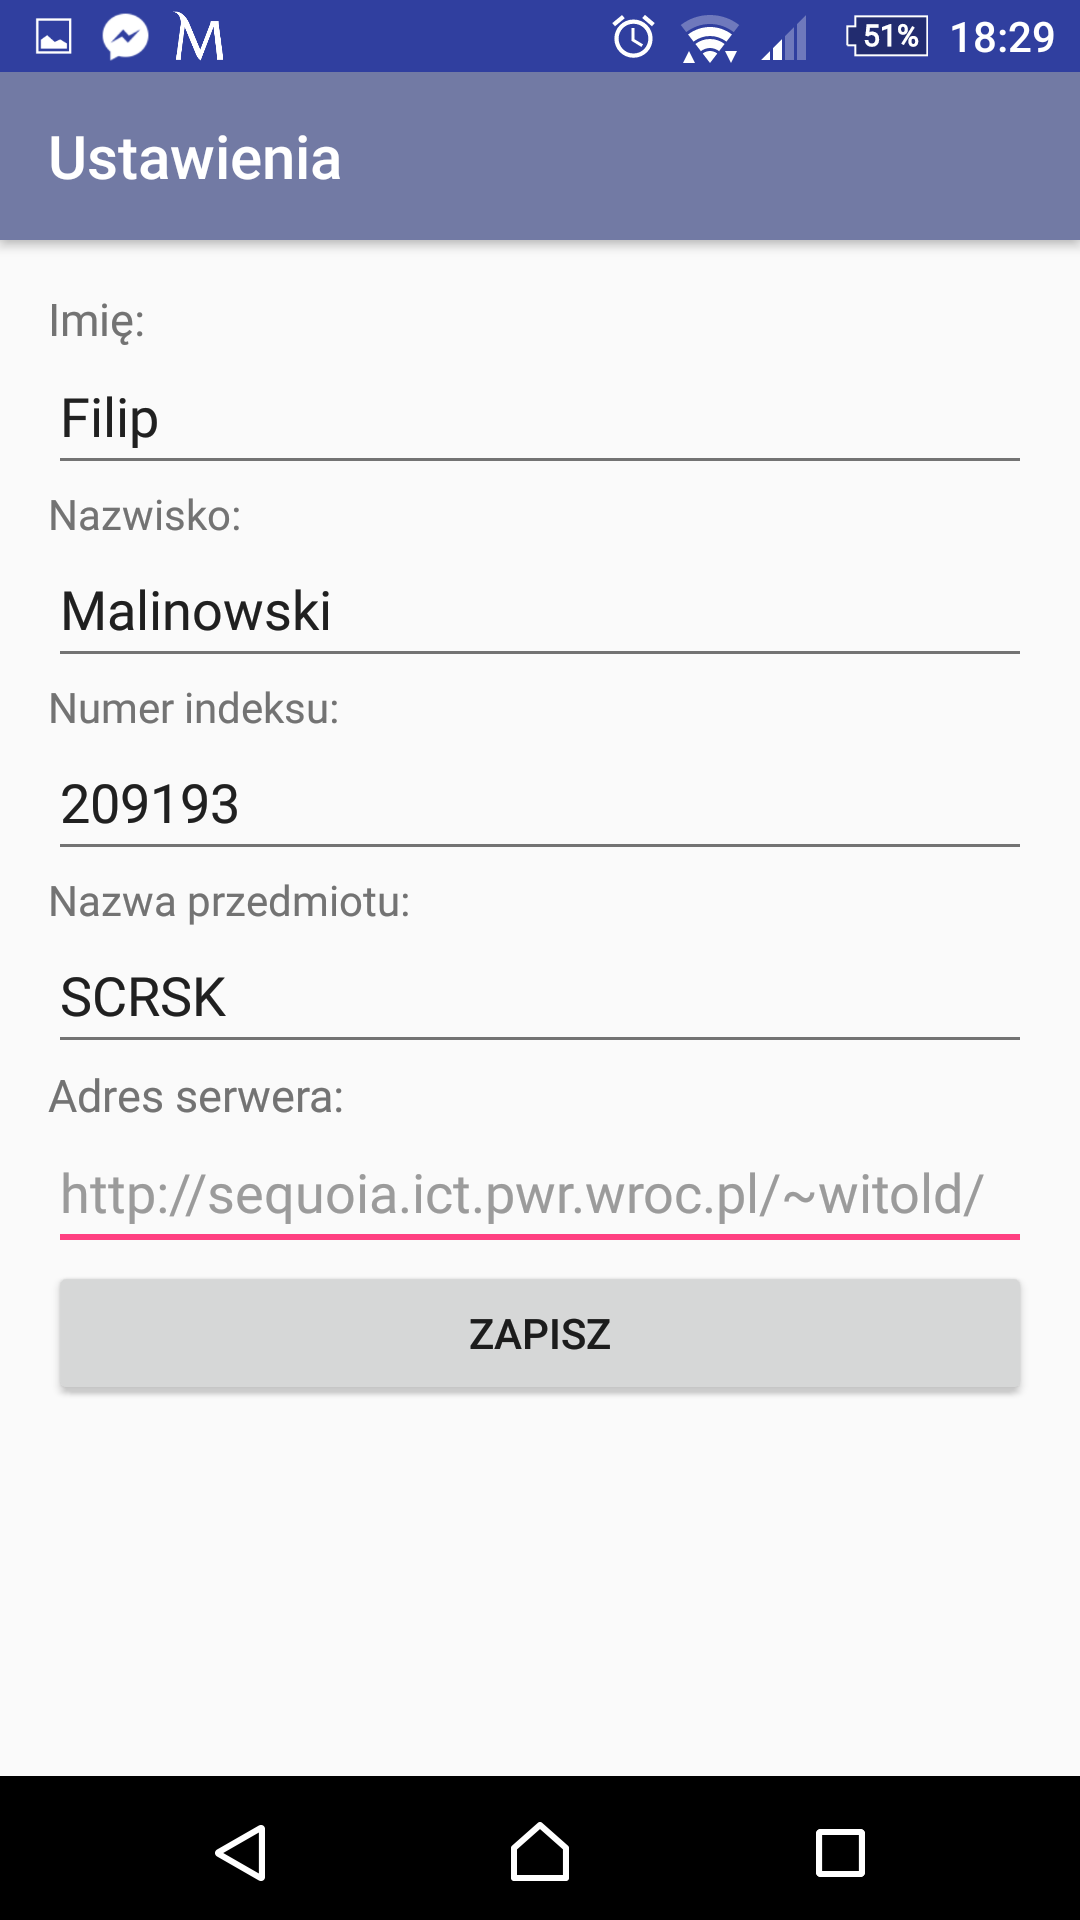
\includegraphics[scale=0.1]{widok_ustawien}
					\end{center}
				\end{figure}
			\end{minipage} \hfill
			
			\item Widok konfigurowania testu\\
			Tutaj użytkownik jest informowany o przebiegu połączenia testowego z serwerem, pobrania pliku konfiguracyjnego, sprawdzeniu poprawności wersji aplikacji oraz sprawdzeniu poprawności otrzymanego klucza szyfrowania.
			
			\item Widok testu\\
			W tym miejscu użytkownik może wybierać odpowiedzi na pytania o danym numerze, dodać kolejne karty, z których może wysłać następne odpowiedzi oraz przejść do podsumowania testu gdzie dowie się w liczbach jakie odpowiedzi wybrał oraz ile z tych odpowiedzi znajduje się w pliku testu na telefonie. Może też wrócić do testu aby go kontynuować lub też go zakończyć wracają co do widoku głównego.
			
		\end{itemize}
		
		\section{Interaktywne elementy na widokach}
		
		W widoku ustawień po kliknięciu na pole do edycji  nazwy testu zastosowano rozwijaną listę z proponowanymi nazwami testów.	W widoku głównym zastosowano podobną listę, która generuje propozycje na podstawie wybranej wcześniej nazwy przedmiotu. Celem było zminimalizowanie błędów popełnianych przez studentów przed testem przy konfigurowaniu aplikacji.
		
		W aplikacji zastosowano również interaktywne elementy sygnalizujące operacje zachodzące w trakcie korzystania z aplikacji.
		Pierwszym z nich jest przycisk o nazwie Android Circular Progress Button\footnote{https://github.com/flavioarfaria/circular-progress-button} został stworzony przez Danylyk Dmytra i udostępniony na licencji MIT. Przycisk ten w aplikacji zmienia swój kolor oraz wygląd sygnalizując:
		\begin{itemize}
			\item bezczynność - niebieski pusty przycisk
			\item przetwarzanie operacji - wirujące kółko
			\item powodzenie przetwarzania operacji - zielony przycisk z checkmark
			\item niepowodzenie przetwarzania operacji - czerwony przycisk 
		\end{itemize}
		Sygnalizowanie bezczynności zostało początkowo użyte dla jednej nieaktywnej funkcji, którą była walidacja aplikacji. Zielony kolor wykorzystany został do sygnalizowania powodzenia połączenia z serwerem oraz do sygnalizowania poprawnego pobrania pliku konfiguracyjnego z walidacją klucza szyfrowania i dopuszczalnej wersji aplikacji.
		Czerwony kolor został wykorzystany do sygnalizowania niepowodzenia wyżej wymienionych operacji.
		Wirujące kółko trwało tak długo jak te asynchronicznie wykonywane operacje nie zakończyły swojego działania.\\
		
		tutaj będą obrazki pokazujące jak zmienia się przycisk\\
		
		Drugim z nich są przyciski występujące na kartach z odpowiedziami w aplikacji. Przyciski te sygnalizują swoimi kolorami etap przetwarzania odpowiedzi użytkownika. Biały przycisk sygnalizuje brak wybranej do tej pory odpowiedzi. Szary przycisk sygnalizuje poprawnie zapisaną odpowiedź do pliku testowego. Niebieski przycisk sygnalizuje poprawnie wysłaną odpowiedź na serwer. Jeżeli operacja zapisywania do pliku się nie powiedzie to przycisk pozostaje biały. Jeżeli operacja wysyłania do serwera się nie powiedzie to przycisk zakolorowywany jest jedynie na szaro informując użytkownika o tym, że ta odpowiedź będzie przechowywana jedynie lokalnie na telefonie.\\
		
		tutaj będą obrazki pokazujące przykładowo wybraną odpowiedź\\
		
		\section{Powiadomienia}
		
		Istotnym elementem aplikacji okazały się być powiadomienia pozwalające na zrozumienie użytkownikowi wydarzeń występujących w aplikacji. Dzięki wypracowaniu zestawu chmurek oraz monitów użytkownik jest informowany o powodzeniu w edycji ustawień aplikacji, błędach występujących przy konfigurowaniu testu oraz różnych innych zdarzeniach takich jak utrata połączenia z serwerem czy też brak poprawnego testu, na który użytkownik chce wysyłać odpowiedzi.
		
	
		\section{Szyfrowanie plików}
	
		Początkowo pliki były szyfrowane algorytmem DES z kluczem generowanym na podstawie łańcucha znaków. Szyfrowało to tekst w dość niezadowalający sposób ujawniając regularności w zakodowanym tekście. Ponadto klucz szyfrowania można było uzyskać po zdekompilowaniu aplikacji. Pierwszym ulepszeniem zaimplementowanym w aplikacji było zastosowanie metody "security by obscurity", gdzie klucz szyfrowania zmieniał się w trakcie działania programu. W ten sposób sprawa jego uzyskania została utrudniona.
		W dalszym etapie wykorzystano szyfrowanie algorytmem RSA. Klucz publiczny jest wykorzystywany w aplikacji do szyfrowania odpowiedzi i zapisywania ich do pliku testu. Uzyskano w ten sposób zadowalający nieregularny wygląd odpowiedzi w pliku testu. Aplikacja została też zmodyfikowana w taki sposób, że klucz publiczny jest pobierany w pliku konfiguracyjnym z serwera pozbywając się niebezpiecznej metody z kluczem bezpośrednio zapisanym w aplikacji.
	
		\section{Skaner QR}
		
		W aplikacji wykorzystano również skaner kodów QR. Jak wcześniej o tym wspomniano, wykorzystano do tego bibliotekę zxing. Pozwala ona nie tylko na skanowanie kodów QR ale również kodów kreskowych, kodów Aztec i innych. Skaner skanuje kod QR wyświetlany na rzutniku  automatyczne wpisując w aplikacji kodu testu, wektor wag. Po operacji wczytywania wymusza wyliczenie nowego numeru grupy. Ułatwia to pracę z aplikacją potencjalnemu użytkownikowi oraz pozwala na zmniejszenie prawdopodobieństwa popełnienia błędu przez użytkownika przy wyliczaniu grupy na teście.
		
		\section{Baza danych}
		
		Do długotrwałego przechowywania danych w aplikacji wykorzystano bazę danych MySQL. W tym celu stworzono klasę imitującą bazę danych MySQL oraz klasę imitującą interfejs dostępowy do tej klasy.
		
		\section{Odrzucanie połączeń w trakcie testu}
		
		W trakcie testowania aplikacji na grupie studentów pojawiła się potrzeba automatycznego odrzucania połączeń. W tym celu stworzono klasę na bazie wbudowanej BroadcastReceiver, która to odrzuca wszystkie przychodzące połączenia o ile użytkownik jest w trakcie pisania testu.
		
	\chapter{Elementy serwera}
		
		\section{Generator konfiguracji}
		
		Generator został napisany w języku Java w wersji pozwalającej uruchomienie go tylko w linii poleceń. W parametrach wywołania tego programu podaje się kod testu, minimalną wersję aplikacji oraz maksymalną wersję aplikacji dopuszczoną do testu. Program generuje dwa pliki. Pierwszy jest dokumentem XML zawierającym minimalną wersję, maksymalną wersję oraz klucz publiczny RSA do szyfrowania odpowiedzi. Drugi plik zawiera klucz prywatny służący do rozszyfrowywania odpowiedzi w pliku z zaszyfrowanymi odpowiedziami na telefonie Android.
		
		\section{Deszyfrator}
		
		Deszyfrator również został napisany w języku Java i umożliwia uruchomienie jedynie w linii poleceń. W parametrach wywołania wprowadza się nazwę pliku z kluczem prywatnym, nazwę pliku z zaszyfrowanymi odpowiedziami i opcjonalnie nazwę pliku wyjściowego. Jeśli zostanie podana nazwa pliku wyjściowego to w nim zostaną zapisane rozszyfrowane odpowiedzi. Bez wybrania nazwy pliku wyjściowego deszyfrator będzie kierować dane na strumień wyjściowy.
		
		\section{Generator kodów QR}
		
		Do generowania slajdów z pytaniami wykorzystano również bibliotekę do generowania kodów QR o nazwie libqrencode\footnote{https://github.com/fukuchi/libqrencode}. Jest to biblioteka napisana w języku C udostępniająca generator kodów oraz pliki nagłówkowe pozwalające na napisanie własnej aplikacji generującej kody QR, Aztec lub inne.
			
\end{document}